
\documentclass[a4paper,11pt]{article}
\usepackage[a4paper, margin=8em]{geometry}

% usa i pacchetti per la scrittura in italiano
\usepackage[french,italian]{babel}
\usepackage[T1]{fontenc}
\usepackage[utf8]{inputenc}
\frenchspacing 

% usa i pacchetti per la formattazione matematica
\usepackage{amsmath, amssymb, amsthm, amsfonts}

% usa altri pacchetti
\usepackage{gensymb}
\usepackage{hyperref}
\usepackage{standalone}

% imposta il titolo
\title{Appunti Fondamenti di Automatica}
\author{Luca Seggiani}
\date{2025}

% disegni
\usepackage{pgfplots}
\pgfplotsset{width=10cm,compat=1.9}

% imposta lo stile
% usa helvetica
\usepackage[scaled]{helvet}
% usa palatino
\usepackage{palatino}
% usa un font monospazio guardabile
\usepackage{lmodern}

% tikz in sans
\tikzset{every picture/.style={/utils/exec={\sffamily}}}

\renewcommand{\rmdefault}{ppl}
\renewcommand{\sfdefault}{phv}
\renewcommand{\ttdefault}{lmtt}

% circuiti
\usepackage{circuitikz}
\usetikzlibrary{babel}

% disponi il titolo
\makeatletter
\renewcommand{\maketitle} {
	\begin{center} 
		\begin{minipage}[t]{.8\textwidth}
			\textsf{\huge\bfseries \@title} 
		\end{minipage}%
		\begin{minipage}[t]{.2\textwidth}
			\raggedleft \vspace{-1.65em}
			\textsf{\small \@author} \vfill
			\textsf{\small \@date}
		\end{minipage}
		\par
	\end{center}

	\thispagestyle{empty}
	\pagestyle{fancy}
}
\makeatother

% disponi teoremi
\usepackage{tcolorbox}
\newtcolorbox[auto counter, number within=section]{theorem}[2][]{%
	colback=blue!10, 
	colframe=blue!40!black, 
	sharp corners=northwest,
	fonttitle=\sffamily\bfseries, 
	title=Teorema~\thetcbcounter: #2, 
	#1
}

% disponi definizioni
\newtcolorbox[auto counter, number within=section]{definition}[2][]{%
	colback=red!10,
	colframe=red!40!black,
	sharp corners=northwest,
	fonttitle=\sffamily\bfseries,
	title=Definizione~\thetcbcounter: #2,
	#1
}

% disponi problemi
\newtcolorbox[auto counter, number within=section]{problem}[2][]{%
	colback=green!10,
	colframe=green!40!black,
	sharp corners=northwest,
	fonttitle=\sffamily\bfseries,
	title=Problema~\thetcbcounter: #2,
	#1
}

% disponi codice
\usepackage{listings}
\usepackage[table]{xcolor}

\lstdefinestyle{codestyle}{
	backgroundcolor=\color{black!5}, 
	commentstyle=\color{codegreen},
	keywordstyle=\bfseries\color{magenta},
	numberstyle=\sffamily\tiny\color{black!60},
	stringstyle=\color{green!50!black},
	basicstyle=\ttfamily\footnotesize,
	breakatwhitespace=false,         
	breaklines=true,                 
	captionpos=b,                    
	keepspaces=true,                 
	numbers=left,                    
	numbersep=5pt,                  
	showspaces=false,                
	showstringspaces=false,
	showtabs=false,                  
	tabsize=2
}

\lstdefinestyle{shellstyle}{
	backgroundcolor=\color{black!5}, 
	basicstyle=\ttfamily\footnotesize\color{black}, 
	commentstyle=\color{black}, 
	keywordstyle=\color{black},
	numberstyle=\color{black!5},
	stringstyle=\color{black}, 
	showspaces=false,
	showstringspaces=false, 
	showtabs=false, 
	tabsize=2, 
	numbers=none, 
	breaklines=true
}

\lstdefinelanguage{javascript}{
	keywords={typeof, new, true, false, catch, function, return, null, catch, switch, var, if, in, while, do, else, case, break},
	keywordstyle=\color{blue}\bfseries,
	ndkeywords={class, export, boolean, throw, implements, import, this},
	ndkeywordstyle=\color{darkgray}\bfseries,
	identifierstyle=\color{black},
	sensitive=false,
	comment=[l]{//},
	morecomment=[s]{/*}{*/},
	commentstyle=\color{purple}\ttfamily,
	stringstyle=\color{red}\ttfamily,
	morestring=[b]',
	morestring=[b]"
}

% disponi sezioni
\usepackage{titlesec}

\titleformat{\section}
{\sffamily\Large\bfseries} 
{\thesection}{1em}{} 
\titleformat{\subsection}
{\sffamily\large\bfseries}   
{\thesubsection}{1em}{} 
\titleformat{\subsubsection}
{\sffamily\normalsize\bfseries} 
{\thesubsubsection}{1em}{}

% disponi alberi
\usepackage{forest}

\forestset{
	rectstyle/.style={
		for tree={rectangle,draw,font=\large\sffamily}
	},
	roundstyle/.style={
		for tree={circle,draw,font=\large}
	}
}

% disponi algoritmi
\usepackage{algorithm}
\usepackage{algorithmic}
\makeatletter
\renewcommand{\ALG@name}{Algoritmo}
\makeatother

% disponi numeri di pagina
\usepackage{fancyhdr}
\fancyhf{} 
\fancyfoot[L]{\sffamily{\thepage}}

\makeatletter
\fancyhead[L]{\raisebox{1ex}[0pt][0pt]{\sffamily{\@title \ \@date}}} 
\fancyhead[R]{\raisebox{1ex}[0pt][0pt]{\sffamily{\@author}}}
\makeatother

\begin{document}

% sezione (data)
\section{Lezione del 13-05-25}

% stili pagina
\thispagestyle{empty}
\pagestyle{fancy}

% testo
\subsection{Sensitività al controllo}
Abbiamo visto le funzioni di \textit{sensitività} $S(s)$ e di \textit{antisensitività} $T(s)$:
$$
S(s) = \frac{1}{1 + L(s)}, \quad T(s) = \frac{L(s)}{1 + L(s)}
$$
Introduciamo adesso un'altra funzione di sensitività, la cosiddetta funzione di \textbf{sensitività al controllo}:
$$
Q(s) = \frac{C(s)}{1 + L(s)}
$$
che vediamo essere la funzione di proporzionalità che ci restituisce il valore del controllo in funzione del riferimento come:
$$
U(s) = \frac{C(s)}{1 + C(s) G(s)} Y_{rif}(s) = Q(s) Y_{rif}(s)
$$

Attraverso la funzione di sensitività al controllo possiamo valutare la conseguenza dell'ingresso di riferimento e/o del disturbo sull'uscita.
Ci consente quindi di inserire nel progetto i vincoli dovuti alle limitazioni fisiche degli attuatori.

\subsubsection{Diagramma di Bode della sensitività al controllo}
Vediamo come tracciare il diagramma di Bode della sensitività al controllo.
Prendiamo il modulo:
$$
|Q(s)| = \frac{|C(j\omega)}{|1 + L(j\omega)|}, \quad s = j\omega
$$
e vediamo i limiti.

\begin{itemize}
	\item A bassa frequenza avremo: 
		$$
		\lim_{\omega \rightarrow 0} |Q(j\omega)| = \frac{|C(j\omega|}{|1 + C(j\omega) G(j\omega)|} \approx \frac{1}{|G(j\omega)|}
		$$
		in quanto $L(S)$ a bassa frequenza è $L(s) >> 0$ (abbiamo detto approssima un integratore);
	\item Ad alta frequenza avremo:
		$$
		\lim_{\omega \rightarrow +\infty} |Q(j\omega)| = \frac{|C(j\omega)|}{|1 + C(j\omega) G(j\omega)|} \approx |C(j\omega)|
		$$
\end{itemize}

Dove per $\omega = \omega_c$:
$$
L(j\omega) = 1 \implies C(j\omega) = \frac{1}{j\omega}
$$

Abbiamo detto che solitamente il sistema si comporta come un passa basso, cioè abbatte oltre una certa frequenza di taglio $\omega_{BP}$.
Avremo allora che:
$$
|G(j\omega)| << 1, \quad \omega \geq \omega_{BP}
$$

Ora, se la frequenza di crossover $\omega_c$ è maggiore della banda del sistema, cioè:
$$
\omega_c > \omega_{BP}
$$
avremo:
$$
|L(j\omega)| > 1, \quad \omega \in (\omega_{BP}, \omega_c)
$$
e quindi riguardo alla sensitività al controllo potremo dire:
$$
|Q(j\omega)| \approx \frac{1}{|G(j\omega)} >> 1, \quad \omega \in (\omega_{BP}, \omega_c)
$$

Questo significa che cercare di aumentare la banda del sistema aumentando la frequenza di crossover conduce a valori di controllo molto elevati e non sempre accettabili: potremmo superare i limiti fisici degli attuatori.
Una regola aurea è di non cercare mai di estendere eccessivamente l'ampiezza di banda dell'impianto.

Quanto detto si traduce in ulteriori vincoli sul diagramma di bode, cioè barriere in alta frequenza sulla funzione di anello e sulla funzione del controllore:
\[
	\begin{cases}
		|L(j\omega)| < \epsilon_u, \quad \omega \geq \omega_u \\
		|C(j\omega)| < \epsilon_{ru}, \quad \omega \geq \omega_{ru}
	\end{cases}
\]

\subsubsection{Esempio: loop shaping della velocità di crociera 2}
Riprendiamo l'esempio della scorsa lezione (27.4.3), e iniziamo a considerare l'effetto di rumori e disturbi.

Oltre ai vincoli già applicati sulla pulsazione minima, quindi, avremo bisogno di vincoli sul guadagno minimo alle basse frequenze (buona reiezione dei disturbi) e sul guadagno massimoa alle alte frequenze (buona reiezione dei rumori), che riportiamo in nero.

\noindent
\begin{minipage}{\textwidth}

Avremo poi bisogno delle barriere di cui abbiamo appena parlato per gli attuatori, alle altre frequenze, che riportiamo in verde, per cui il grafico complessivo risulterà una cosa del tipo:
\begin{center}
	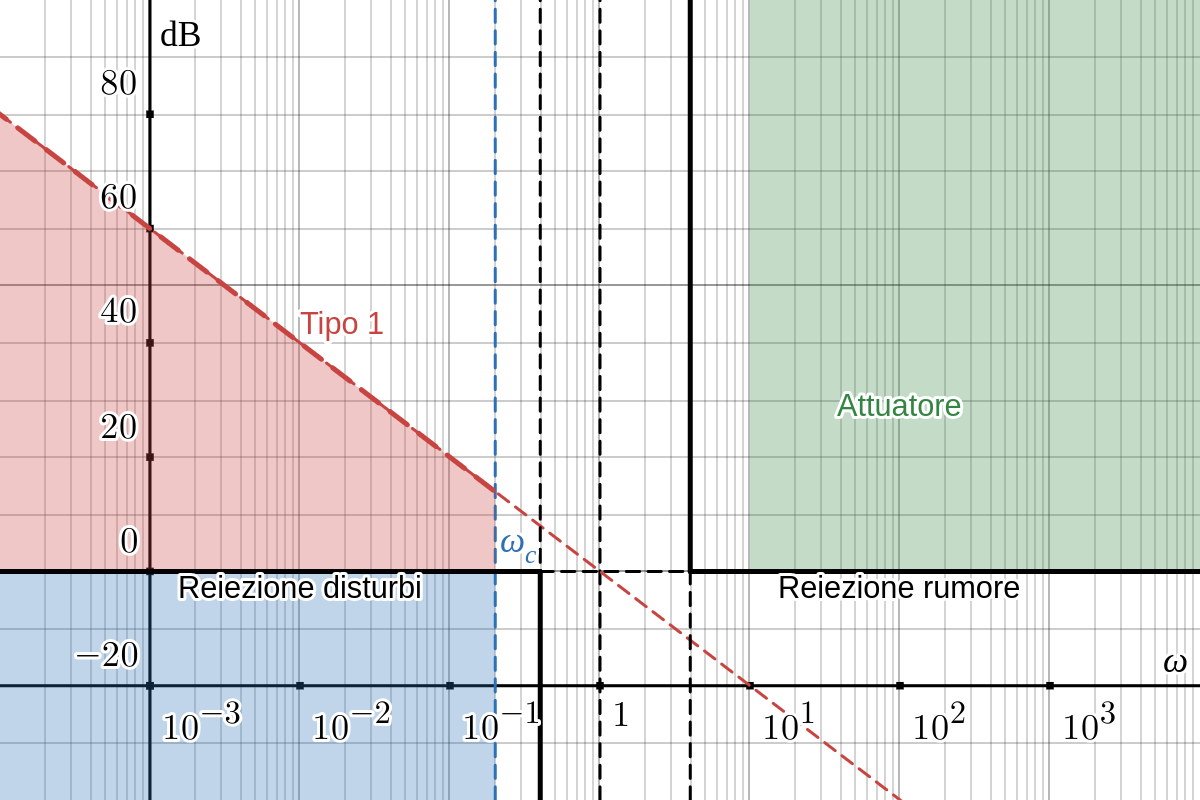
\includegraphics[scale=0.28]{../figures/crociera_full_regions.png}
\end{center}

\end{minipage}

Notiamo quindi di avere una grande quantità di vincoli di cui tener conto, molti dei quali si sovrappongono fra di loro.
Abbiamo infatti che una serie di specifiche troppo stringenti possono rendere difficile o impossibile il progetto del sistema di controllo.
Bisogna verificare sempre che le specifiche richieste siano compatibili col problema: e meglio comprare sensori migliori che impegnarsi nel progetto di un regolatore con specifiche troppo esigienti.

\end{document}
